
\begin{figure}[H]
\centering

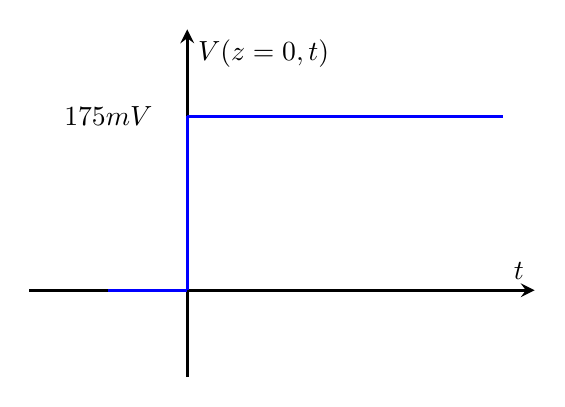
\begin{tikzpicture} 
\begin{axis}[very thick,
                     samples = 100,
                     ytick={-2,2},
                     xlabel = {$t$},
                     ylabel = {$V(z=0, t)$},
                     xmin = -1,
                     xmax = 2.2,
                     ymin = -0.5,
                     ymax = 1.5,
                     width=8cm,
                     height=6cm,
                     axis x line = middle,
                     axis y line = middle,
                     ticks = none]
                     
            \addplot[blue] coordinates {(-0.5,0) (0,0)};
            \addplot[blue] coordinates {(0,0) (0,1)};
            \addplot[blue] coordinates {(0,1) (2,1)};
            \node at (axis cs:-0.5,1){$175 mV$};
            
        \end{axis}
\end{tikzpicture}

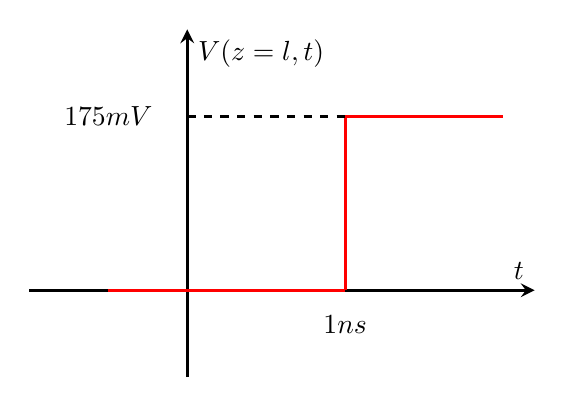
\begin{tikzpicture} 
\begin{axis}[very thick,
                     samples = 100,
                     ytick={-2,2},
                     xlabel = {$t$},
                     ylabel = {$V(z=l, t)$},
                     xmin = -1,
                     xmax = 2.2,
                     ymin = -0.5,
                     ymax = 1.5,
                     width=8cm,
                     height=6cm,
                     axis x line = middle,
                     axis y line = middle,
                     ticks = none]
                     
            \addplot[red] coordinates {(-0.5,0) (1,0)};
            \addplot[red] coordinates {(1,0) (1,1)};
            \addplot[red] coordinates {(1,1) (2,1)};
            \addplot[dashed] coordinates {(0,1) (1,1)};
            \node at (axis cs:-0.5,1){$175 mV$};
            \node at (axis cs:1,-0.2){$1ns$};
            
        \end{axis}
\end{tikzpicture}

\caption{First graph shows the voltage at the start of the line and the second shows the voltage at the end of the line. Source: own.}
\label{graph:1} 
\end{figure}